\documentclass[12pt,twoside]{article}

% La extensión total de la memoria deberá ser de un máximo de 50 páginas (excluidos resumen, índice y posibles anexos).

% Según las recomendaciones de estilo, el formato de la memoria se ajustará a lo siguiente:
% ? Formato del papel: DIN A4.
% ? Impresión a dos caras.
% ? Márgenes: superior e inferior, 2.5 cm. Márgenes laterales: páginas impares, izquierdo 4 cm y derecho 2 cm; páginas % pares, izquierdo 2 cm y derecho 4 cm.
% ? Tipo de letra: Times New Roman de 12 puntos.
% ? Interlineado: 1.5 líneas.
% ? Alineación: justificación completa.
% ? Sangrado de párrafo: 0.5 cm la primera línea de cada párrafo. No se
%pondrá espacio entre párrafos.
% ? Las páginas deberán ir numeradas en números arábigos.

% Teniendo en cuenta las indicaciones previas, definimos el estilo en LaTeX:

% Indicaciones para el idioma:
\usepackage[T1]{fontenc}
\usepackage[utf8]{inputenc}
\usepackage[spanish]{babel}
\usepackage{float}

% Adaptación de itemize y enumerate a los usos tipograficos españoles:
\let\layoutspanish\relax
\addto\captionsspanish{\def\tablename{Tabla}} % para que escriba "Tabla" en lugar de "Cuadro"
\unaccentedoperators  % para que no acentúe los operadores

% Área de impresión de una página:
\usepackage[a4paper]{geometry}
  \geometry{hmargin={2.5cm,2.5cm},height=22cm}

% Formato de algunas distancias:
\renewcommand{\baselinestretch}{1.2}    % separación entre líneas de un mismo párrafo
\setlength{\partopsep}{0pt}
\setlength{\itemsep}{0pt}
\setlength{\topsep}{0pt}
\setlength{\parsep}{0pt}
\setlength{\parskip}{0.25\baselineskip}   % separación entre párrafos

\renewcommand{\textfraction}{0.1}   % mínima fracción de la página para el texto
\renewcommand{\topfraction}{1}      % máxima fracción de la página para objetos flotantes en la parte superior
\renewcommand{\bottomfraction}{1}
\renewcommand{\floatpagefraction}{1}

\setcounter{totalnumber}{5}
\setcounter{topnumber}{3}
\setcounter{bottomnumber}{2}

% Adaptación de las "caption" de los entorns "figure" y "table":
\usepackage{caption}
\setcaptionwidth{\textwidth}
\addtolength{\captionwidth}{-2\parindent}
\captionsetup{margin=\leftmargini,%
  width=\captionwidth,%
  labelfont={up,bf},%
  font={small,sl},%
  %indention={\captionindent
}

% Indentación del primer párrafo de una sección:
\usepackage{indentfirst}

% Definición del color grisclaro en la salida PDF:
\usepackage[pdftex]{color}

% Gráficos:
\usepackage[pdftex]{graphicx}

% Paquetes recomendados para la inclusión de fórmulas matemáticas:
\usepackage{amsmath}
\allowdisplaybreaks  % para que pueda partir fórmulas que ocupan más de una línea, necesita el paquete anterior
\usepackage{amssymb} % para cargar algunos símbolos como \blacksquare y \square
\usepackage{amsfonts} % para cargar algunas fuentes en estilo matemático
\usepackage{enumerate}
\usepackage{hyperref}
% Teoremas (se pueden definir todos los que se necesiten):


\newtheorem{theorem}{Teorema}[section]
\newtheorem{proposition}[theorem]{Proposición}
\newtheorem{definition}[theorem]{Definición}
\newtheorem{lemma}[theorem]{Lema}
\newtheorem{corollary}[theorem]{Corolario}
\newtheorem{example}[theorem]{Ejemplo}
\newtheorem{app}[theorem]{Aplicación}
\newtheorem{remark}[theorem]{Observación}
\newtheorem{agrad}[theorem]{Agradecimiento}
\newtheorem{algo}[theorem]{Algoritmo}
\newtheorem{axiom}[theorem]{Axioma}
\newtheorem{case}[theorem]{Caso}
\newtheorem{conclu}[theorem]{Conclusión}
\newtheorem{conjectura}[theorem]{Conjetura}
\newtheorem{notac}[theorem]{Notación}
\newtheorem{soluc}[theorem]{Solución}
\newtheorem{summary}[theorem]{Sumario}

\newtheorem{proof}[theorem]{Demostración.}
\renewenvironment{proof}{\textbf{\emph{Demostración.}}} {\quad \hfill $\blacksquare$ \newline} % para que aparezca un cuadrado negro al acabar la demostración


% Definición de cabeceras y pies de página:

\usepackage{fancyhdr}                     % para definir distintos tipos de cabeceras y pies de página

\newcommand{\RunningAuthor}{Adán Avilés Cahill}
\newcommand{\Author}[1]{\renewcommand{\RunningAuthor}{#1}}
\renewcommand{\leftmark}{\RunningAuthor}

\newcommand{\RunningTitle}{Hacking Ético}
\newcommand{\Title}[1]{\renewcommand{\RunningTitle}{#1}}
\renewcommand{\rightmark}{\RunningTitle}


\pagestyle{fancy}
\fancyhf{}
\fancyhead[LO]{\small \slshape \leftmark}    % lo que aparece en la parte izquierda de la páginas impares
\fancyhead[RE]{\small \slshape \rightmark}   % lo que aparece en la parte derecha de las páginas pares
\fancyhead[RO,LE]{\small \slshape \thepage}  % el número de página aparece en la parte exterior de la cabecera
\newcommand{\comment}[1]{}
\renewcommand{\headrulewidth}{0.6pt}         % grueso de la línea horizontal por debajo de la cabecera de la página
\renewcommand{\footrulewidth}{0pt}           % grueso de la línea horizontal por encima del pie de página
                                             % en este caso está vacío
\setlength{\headheight}{1.5\headheight}      % aumenta la altura de la cabecera en una parte y media

\fancypagestyle{plain}{%                     % redefinición del estilo de página 'plain'
  \fancyhf{}                                 % limpia todas las cabeceras y pies de página
  \setlength{\headwidth}{\textwidth}
  \fancyfoot[C]{\small \slshape \thepage}    % excepto el centro del pie de página
  \renewcommand{\headrulewidth}{0pt}
  \renewcommand{\footrulewidth}{0pt}
  }

% Instrucciones que se usan frecuentemente
\newcommand{\abs}[1]{\ensuremath{|#1|}}
\newcommand{\norm}[1]{\left\lVert#1\right\rVert} %norma
\newcommand{\normd}[1]{\left\lVert#1\right\rVert_{2}} %norma
\newcommand{\hil}{\mathcal{H} }
\newcommand{\prodes}[2]{\langle #1, #2 \rangle }
\newcommand{\suc}{\{x_n\}_{n=1}^{\infty}}
\newcommand{\sumi}[2]{\sum_{#1}^{#2}}
\newcommand{\luno}{L^1(\mathbb{R})}
\newcommand{\ldos}{L^2(\mathbb{R})}
\newcommand{\tf}[3]{\dfrac{1}{\sqrt{2 \pi}} \int_{-\infty}^{\infty} #1 e^{-iw#2}d#3}
\newcommand{\erre}{\mathbb{R}}
\newcommand{\intif}{ \int_{-\infty}^{\infty}}
\newcommand{\cdos}{\mathcal{C}_{00}^{2} (\mathbb{R}) }
\newcommand{\tfd}{\mathcal{F}}

% Datos del trabajo y autor:
\title{Práctica Hacking Ético}
\author{Adán Avilés Cahill\\*[1em]
\begin{minipage}{0.75\textwidth}
\footnotesize \itshape
\begin{center}
IMF BUSINESS SCHOOL\\
Máster en Ciberseguridad
\end{center}
\end{minipage}
}
\date{Junio 2014}

% Para incluir paginas de otro pdf (por ejemplo, la de la portada):
\usepackage{pdfpages}

\setlength{\abovedisplayskip}{5pt}
\setlength{\belowdisplayskip}{5pt}

\pagestyle{fancy}
%----------------------------------------------------------------------------------
%-                                  DOCUMENT START                                -
%----------------------------------------------------------------------------------
\begin{document}
\begin{figure}[t]
 \begin{picture}(140,50) \put(140,0){
\includegraphics[width=60mm]{./imagenes/logo-imf-alta}} \end{picture}
\end{figure}

\title{Seguridad en Smartphones}
\author{Adán Avilés}
\date{Octubre 2021}
\maketitle


% A continuación, se incluirá el índice del trabajo y, seguidamente, se desarrollará la memoria.
\newpage
\tableofcontents
\newpage

% ------------------------------------------------- % 
% -          Planteamiento del trabajo            - %
% ------------------------------------------------- % 
\section{Presentación del problema}
A lo largo de los contenidos se ha hablado de OWASP, análisis estático y análisis dinámico,  vulnerabilidades, desarrollo seguro, etc. Los Smartphones no quedan libres de ataques. OWASP define un top 10 de riesgos en aplicaciones para dispositivos móviles, como podemos ver en \url{https://www.owasp.org/index.php/Mobile_Top_10_2016-Top_10}.\\
A partir de los contenidos estudiados y tras leer el enunciado anterior, analiza al menos tres aplicaciones (ficheros .apk) en busca de vulnerabilidades. Para ello utilizaremos \begin{itemize}
    \item Una apk no oficial, con vulnerabilidades deliberadamente introducidas, y que se publican en internet para prácticas de entrenamiento, \textbf{InsecureBankV2}.
    \item Una descargada de algún repositorio no oficial de apks, \textbf{MyFitnessPal free premium}.
    \item Una descargada desde una tienda oficial, \textbf{Instagram}.
\end{itemize}
Para hacer este trabajo se han usado disintas herramientras como
\begin{itemize}
    \item MobSF
    \item ADB (Android Debug Bridge)
    \item Distintas páginas online como VirusTotal o Quixxi
    \item Kali Linux
    \item Santoku
    \item Genymotion 
\end{itemize}

\newpage
% ------------------------------------------------- % 
% -          Análisis de InsecureBankV2           - %
% ------------------------------------------------- % 
\section{Análisis de InsecureBankV2}
Cargaremos la apk en MobSF, para poder hacer los análisis:
\begin{figure}[H]
    \centering
    \fbox{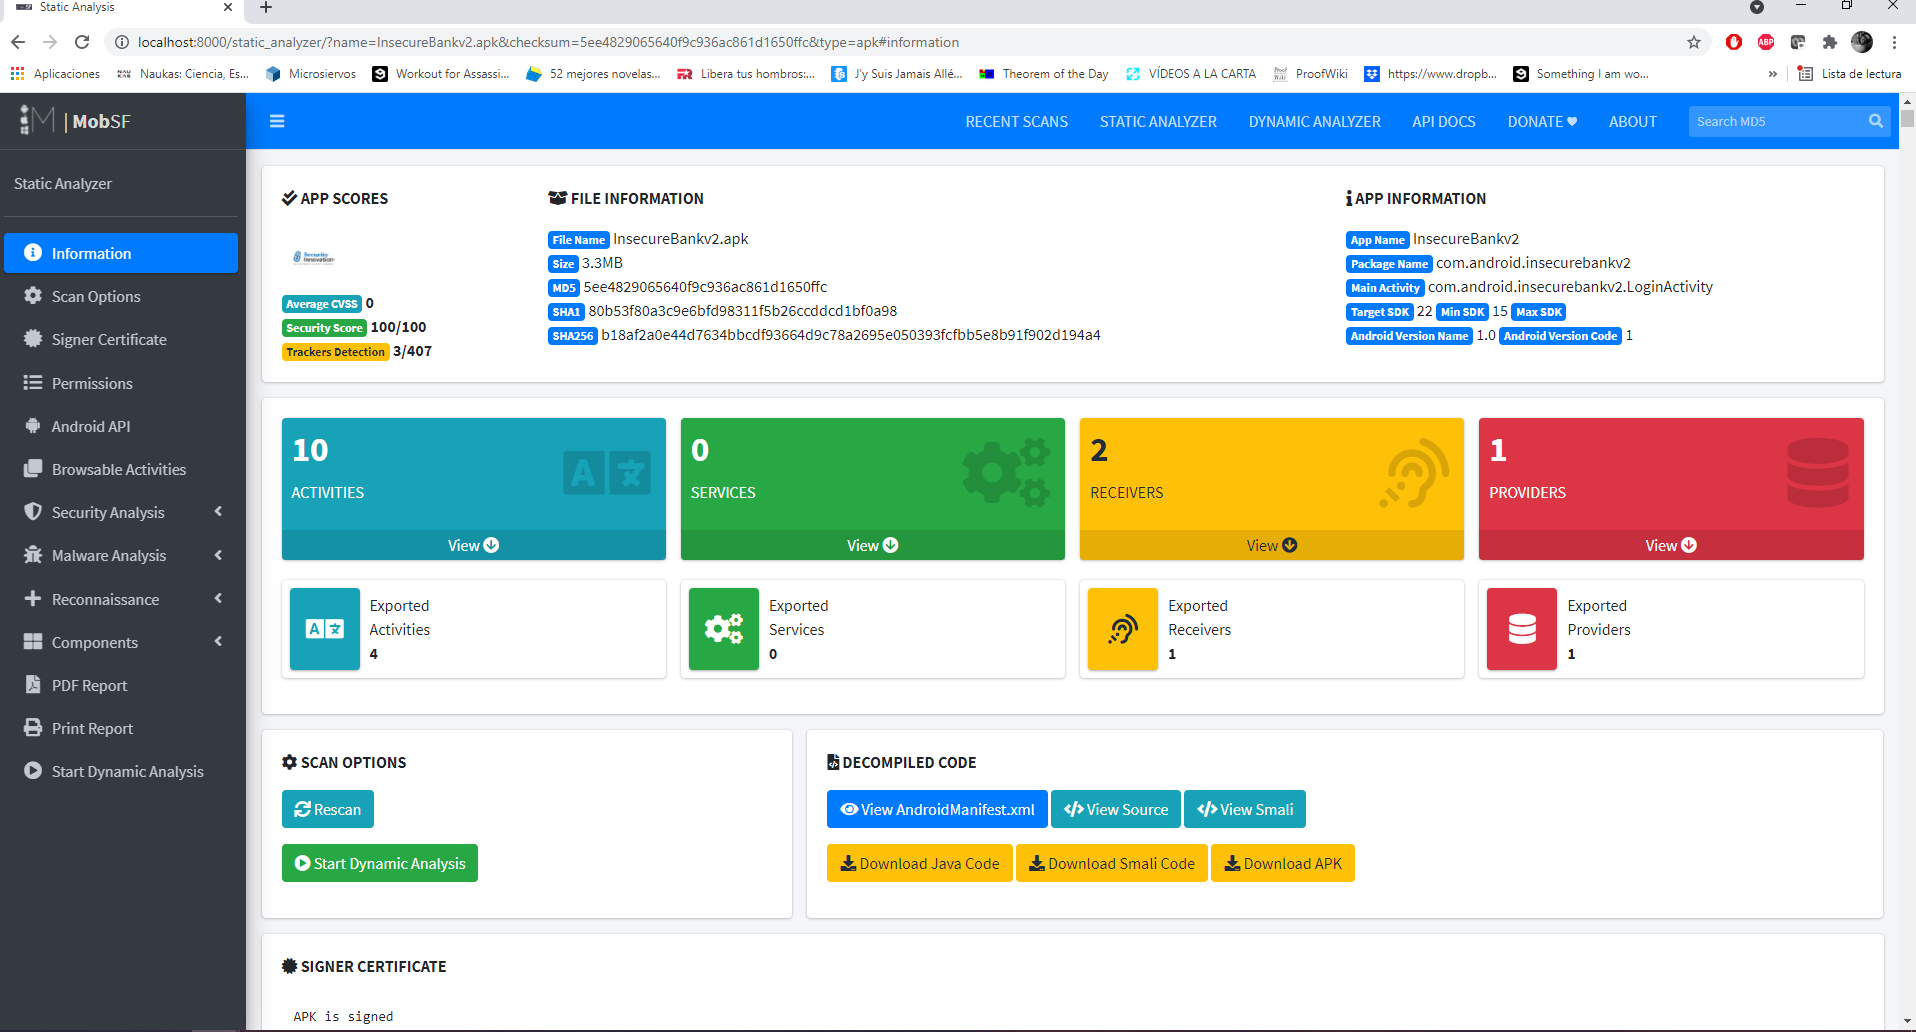
\includegraphics[scale=0.3]{./imagenes/mobsf_ae_insecurebank}}
    \caption{Imagen inicial del análisis estático de MobSF}
\end{figure}
también podemos utilizar herramientas online como \textit{virustotal}
\begin{figure}[H]
    \centering
    \fbox{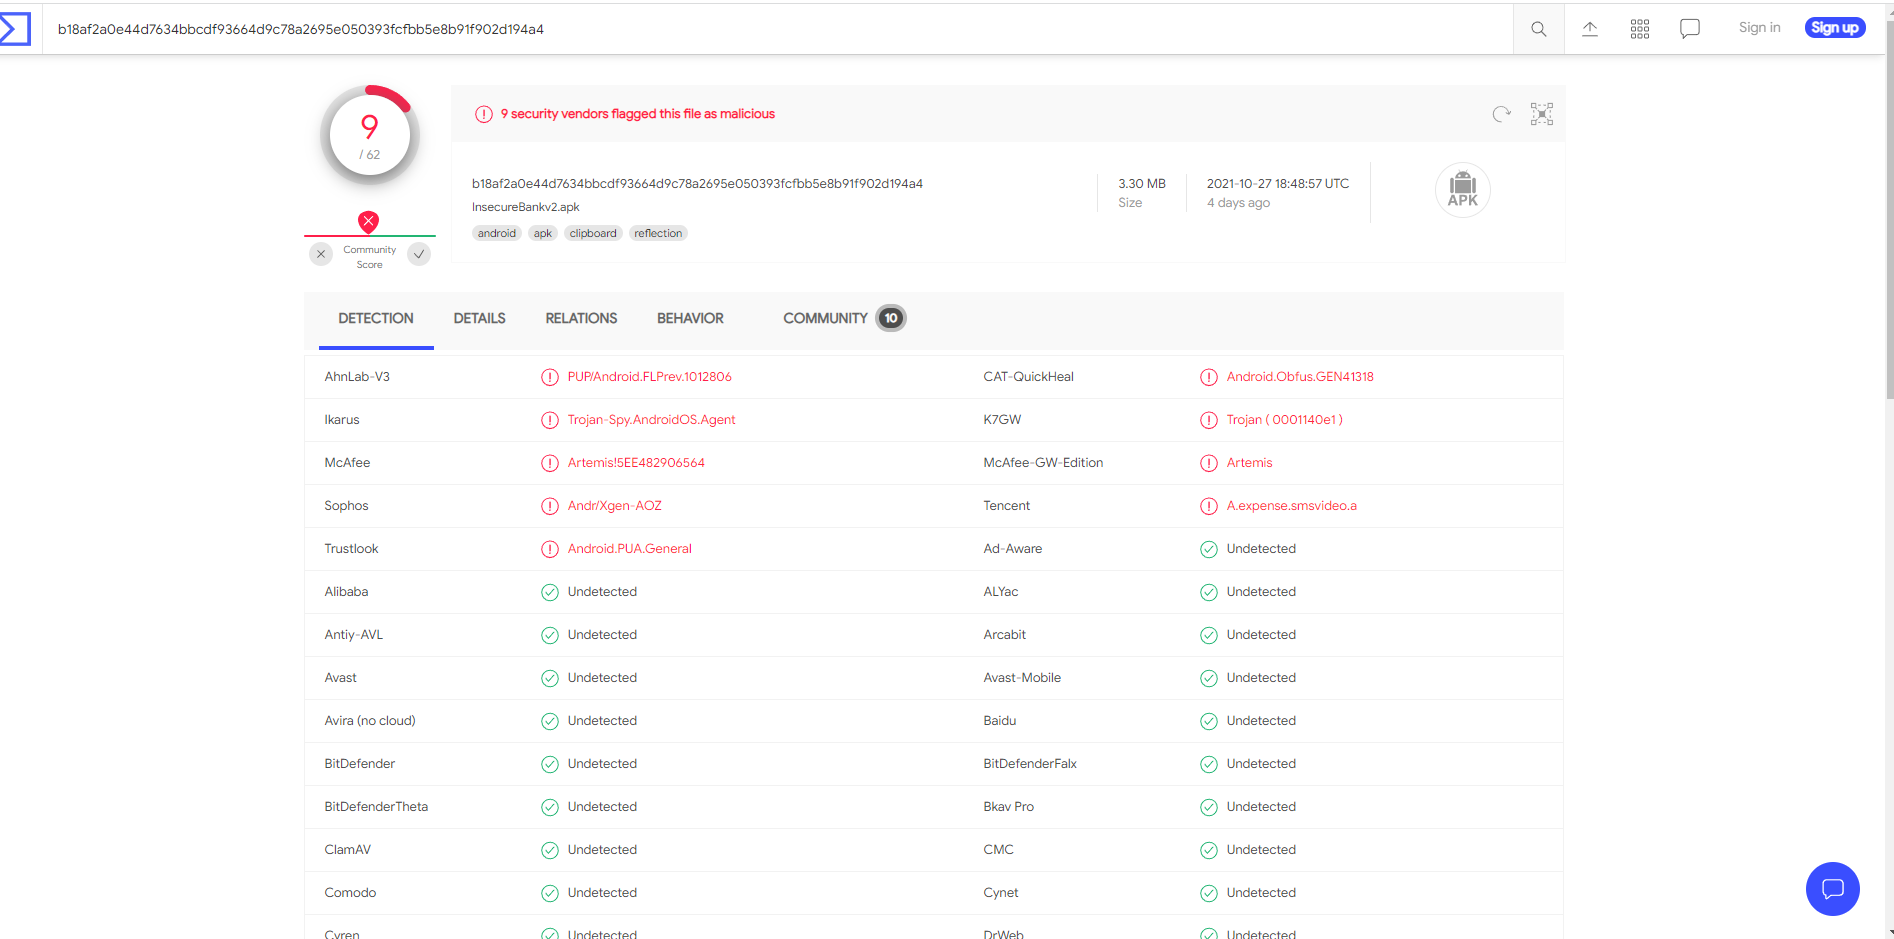
\includegraphics[scale=0.3]{./imagenes/virustotal_insecurebank}}
    \caption{Análisis con VirusTotal}
\end{figure}
\textit{Intezer}
\begin{figure}[H]
    \centering
    \fbox{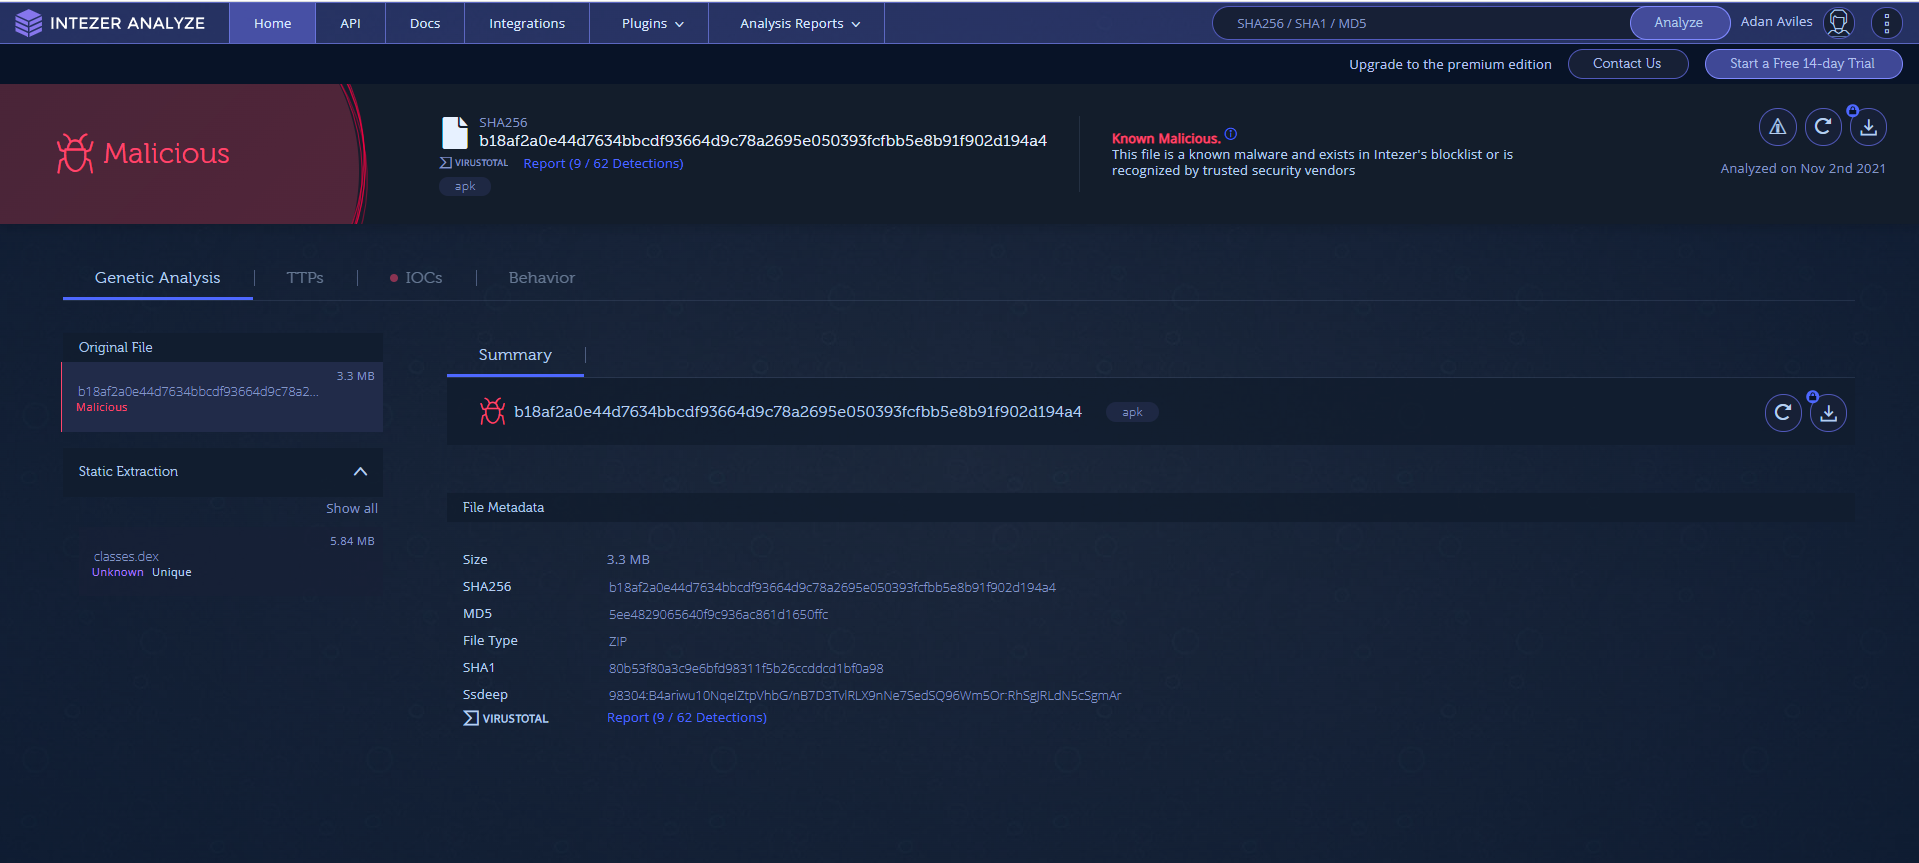
\includegraphics[scale=0.3]{./imagenes/intezer_insecurebank}}
    \caption{Análisis con Intezer}
\end{figure}
\textit{Quixxi}
\begin{figure}[H]
    \centering
    \fbox{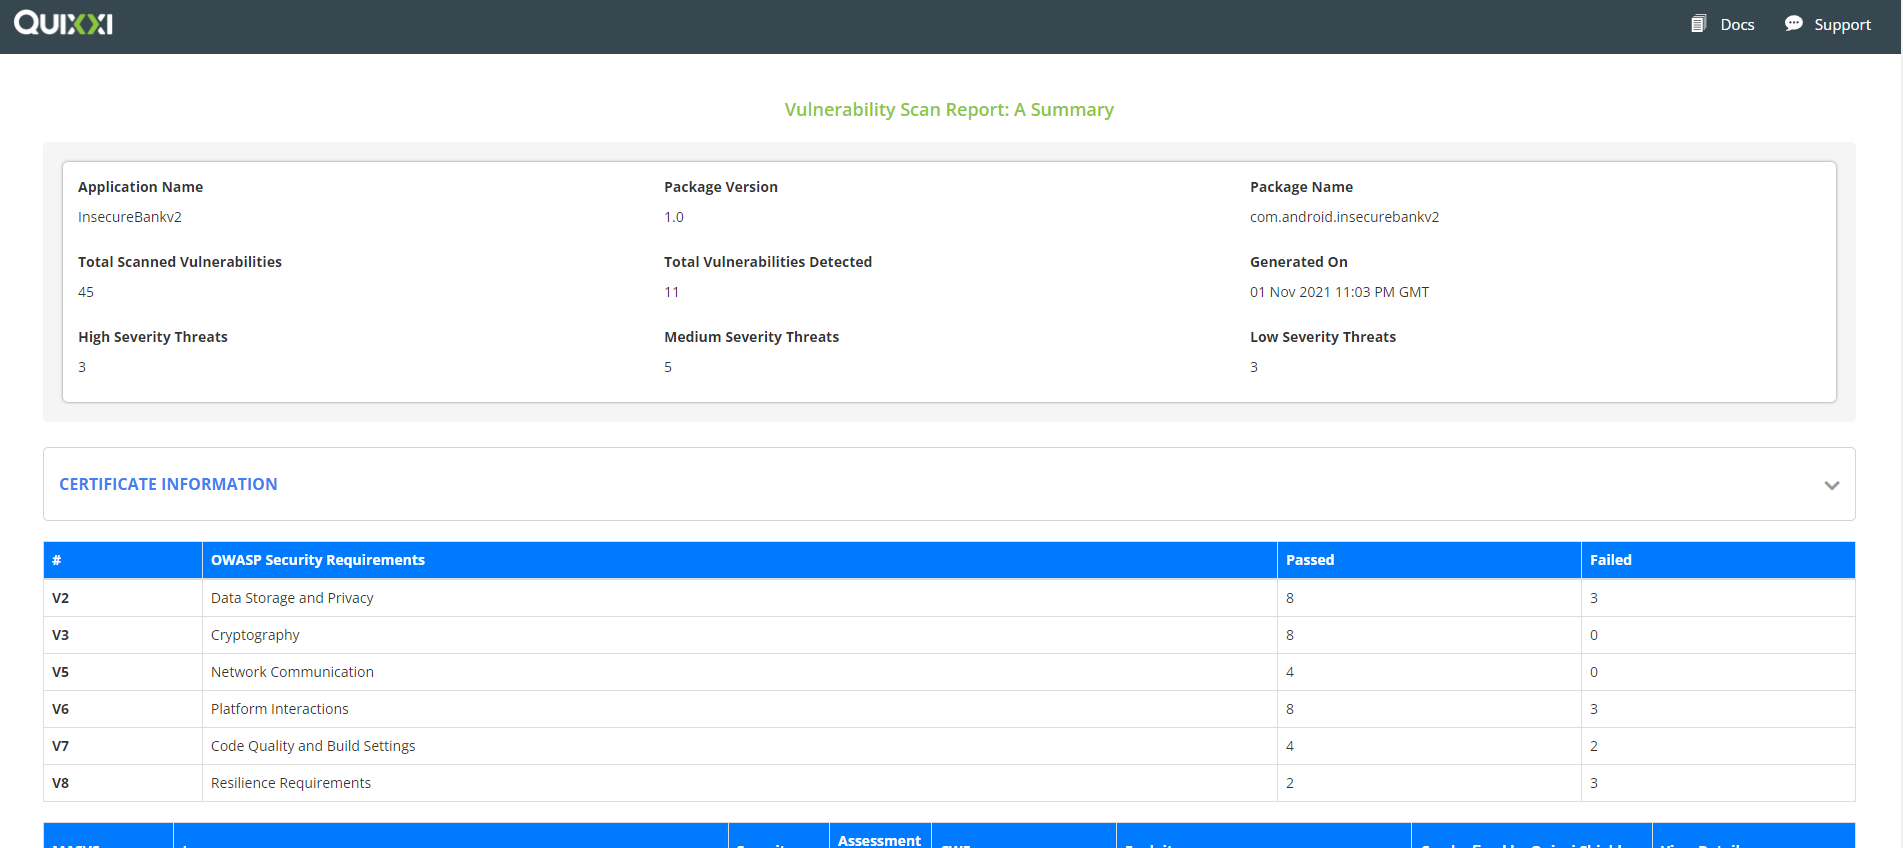
\includegraphics[scale=0.3]{./imagenes/quixxi_insecurebank}}
    \caption{Análisis con Quixxi}
\end{figure}
% ------------------------------------------------- % 
\subsection{Análisis estático}
\subsubsection{Permisos}
Revisaremos en primer lugar el AndroidManifest.xml para ver los permisos.
\begin{figure}[H]
    \centering
    \fbox{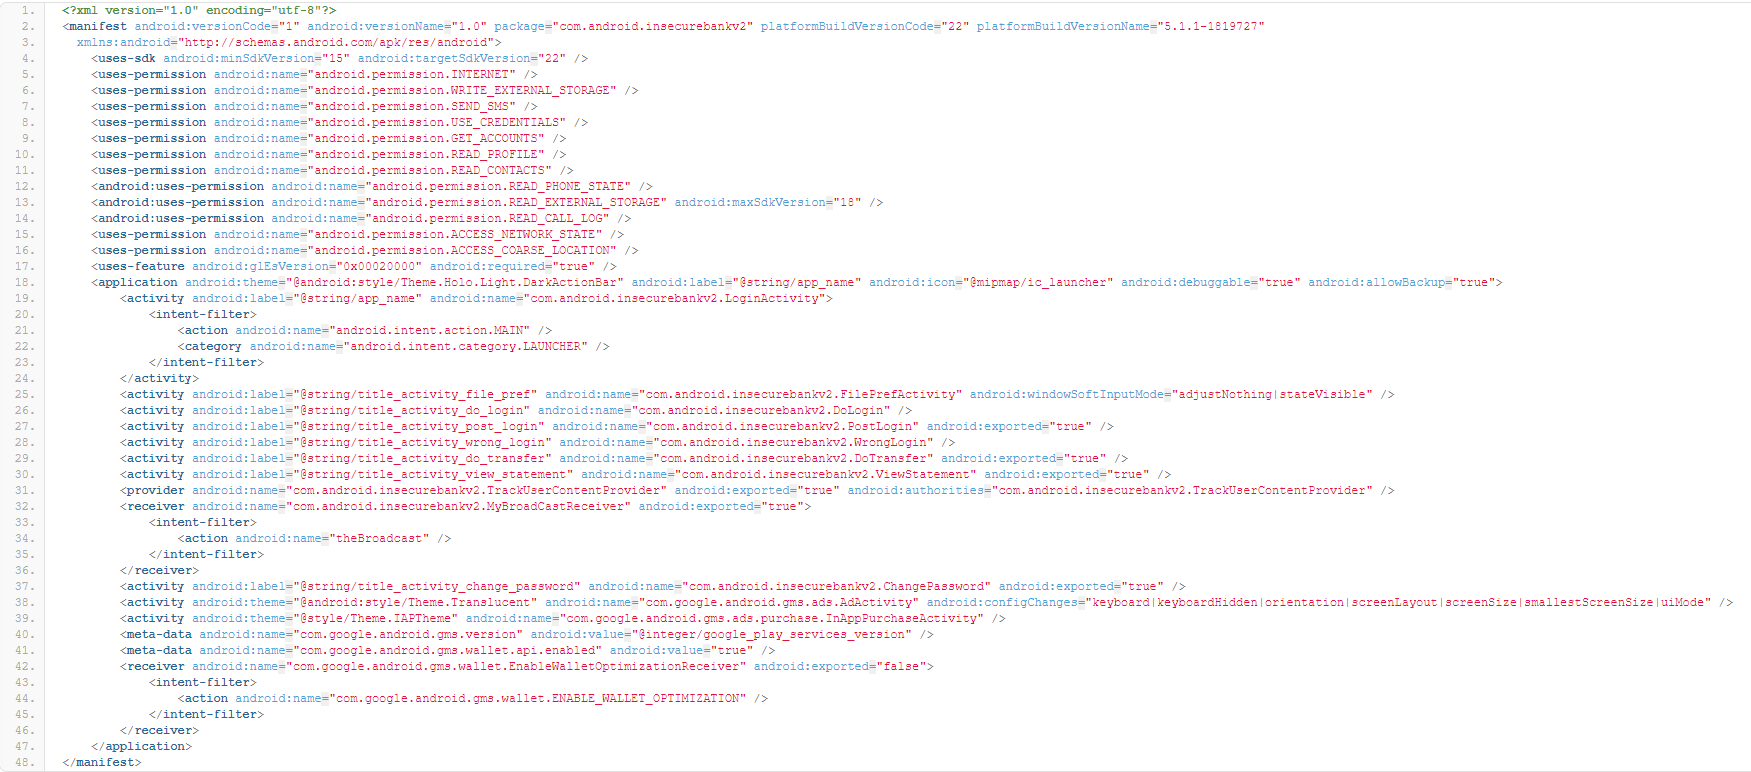
\includegraphics[scale=0.3]{./imagenes/insecurebank_androidmanifest}}
    \caption{AndroidManifest.xml de InsecureBank}
\end{figure}
Listaremos, a continuación, los permisos que pueden ser más peligrosos:
\begin{itemize}
    \item \textbf{SEND\_SMS}: Este permiso, le dará a la app la capacidad de enviar mensajes SMS, que pueden suponer un coste para el usuario.
    \item \textbf{ACCESS\_COARSE\_LOCATION}: Da permisos para obtener la ubicación aproximada a través de la ubicación de  red. 
    \item \textbf{GET\_ACCOUNTS}: Permite a la aplicación obtener las cuentas conocidas almacenadas en el teléfono, como por ejemplo cuentas creadas por otras aplicaciones, es decir, podría obtener nuestros usuarios de otras aplocaciones.
    \item \textbf{READ\_CONTACTS}: Podrá leer los contactos almacenados en el teléfono, llamadas, correos enviados.... Esto permitiría que pueda recabar los datos del usuario y robarlos.
    \item \textbf{READ\_PROFILE}: Lee los datos del usuario. 
    \item \textbf{READ\_LOG}: Lee los datos del usuario.
    \item \textbf{ALLOW\_BACKUP}: Permite realizar BackUps de la aplicación
    \item \textbf{USE\_CREDENTIALS}: Permitirá a la aplicación solicitar tokens de autenticación. 
    \item \textbf{WRITE\_EXTERNAL\_STORAGE}: Permite a la apicación escribir en el almacenamiento externo.
\end{itemize}
\subsubsection{Actividades}
Sabemos que si un componente está exportamos  en el AndroidManifest.xml,cualquier aplicación puede acceder a él si tiene los permisos adecuados. Así, hemos de tener cuidado con las acitivdades que exportamos, por ejemplo, \textbf{PostLogin}\\
Esta actividad puede ser usada en cualquier momento, así que si la ejecutamos, podemos evitar el tener que acceder con usuario y contraseña. También se puede hacer lo mismo con \textbf{DoTransfer} para acceder a las transferencias sin logging. (OWASP M6)
\begin{figure}[H]
    \centering
    \fbox{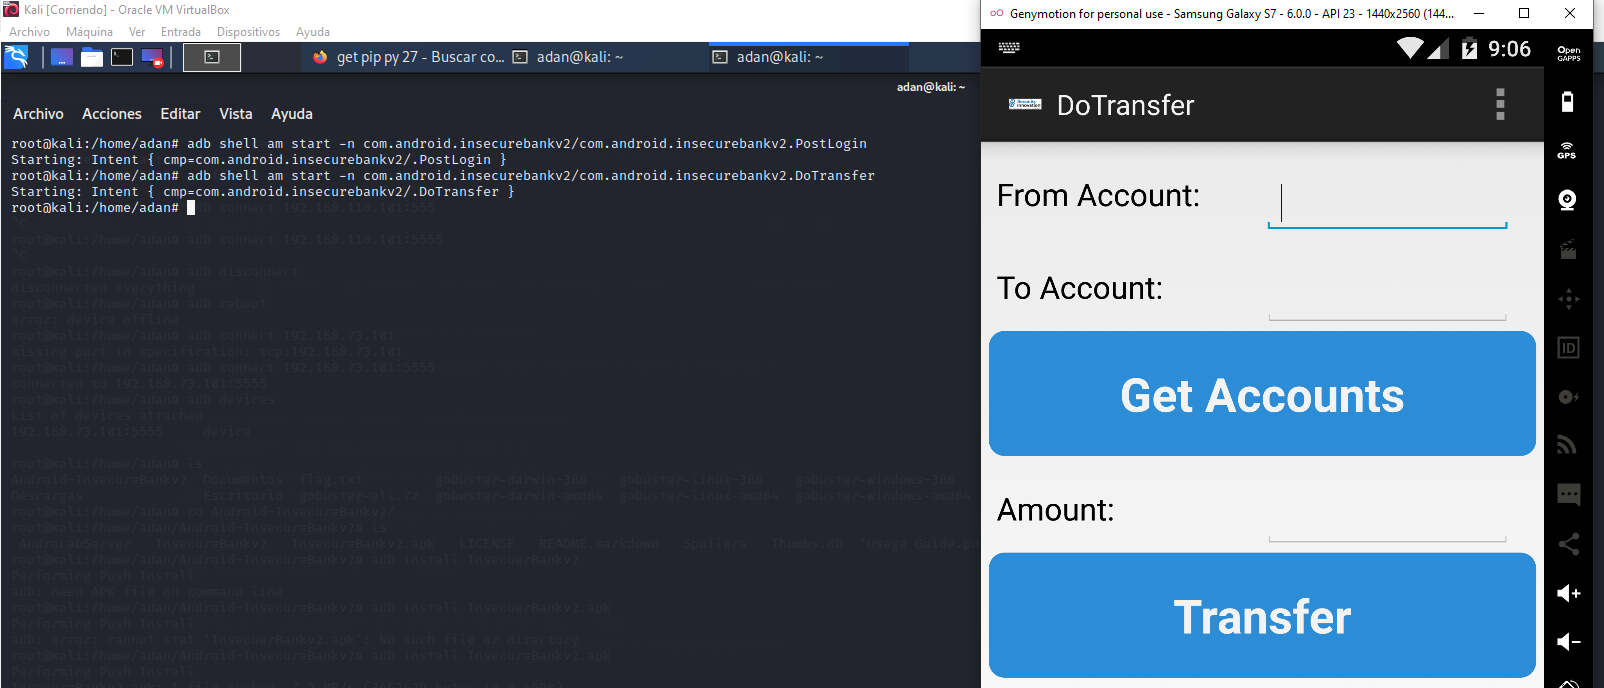
\includegraphics[scale=0.35]{./imagenes/analisisdinamico_1}}
    \caption{Acceso a transferencias}
\end{figure}
Por otro lado, y con los mismos problemas, estarían las actividades de
\begin{itemize}
    \item ChangePassword
    \item ViewStatement
    \item LoginActivity
\end{itemize}
\subsubsection{Receivers}
Encontramos que \textbf{MyBroadCastReceiver} es accesible por otras aplicaciones y realiza la acción \textbf{theBroadcast}. Si revisamos el código, vemos que está relacionado con el cambio de contraseña, y que esta está encriptada en Base64 (OWASP M5), lo cuál no es demasiado seguro. Además, podemos ver que su última orden es enviar un SMS, el atacante podría utilizar esto para robar dinero en forma de mensajes SMS sin el consentimiento del usuario.
\begin{figure}[H]
    \centering
    \fbox{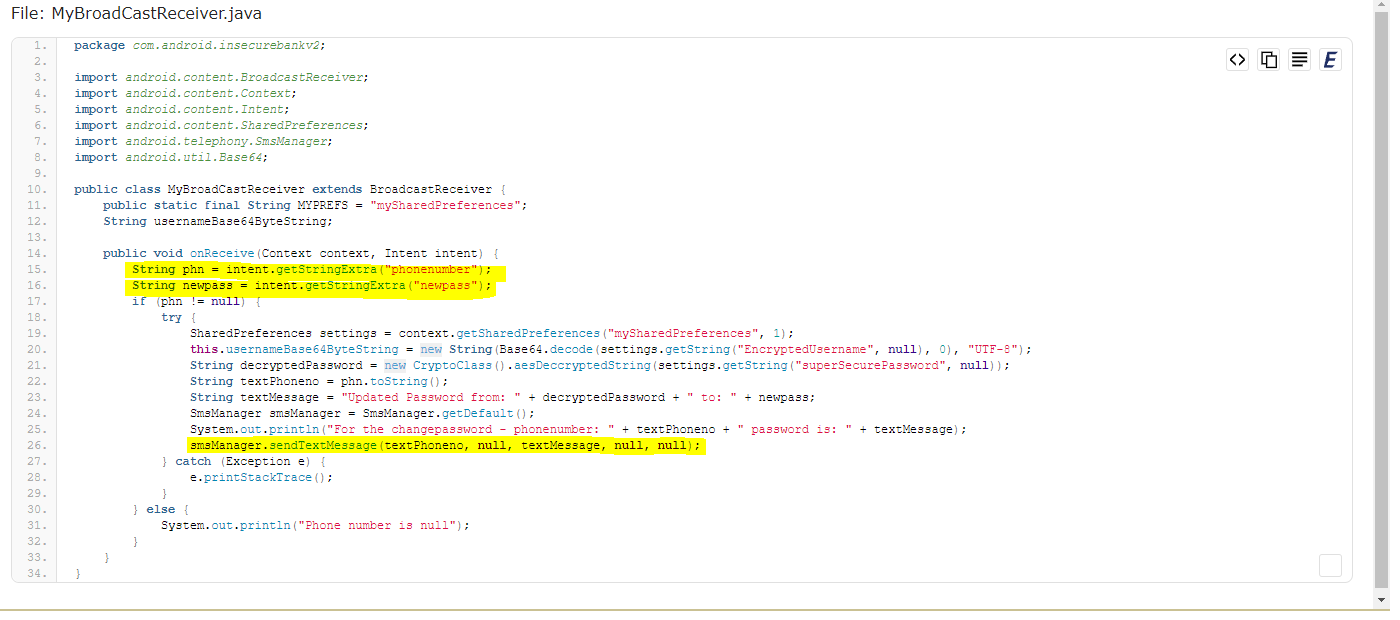
\includegraphics[scale=0.4]{./imagenes/mybroadcastreceiver}}
    \caption{Código de MyBroadcastReceiver}
\end{figure}

\subsubsection{ContentProvider}
El contentprovider \textbf{TrackUserContentProvider} no está protegido por ningún permiso, lo cuál puede hacer que sea vulnerable a ataques de SQL injection. 

\subsubsection{Almacenamiento de las credenciales}
Este paso también se podría revisar en el análisis dinámico, pero lo haremos revisando el código. La aplicación permite la opción del \textit{autofill} de credenciales, que estarán almacenadas en algún lugar.
Buscaremos en el código de \textit{DoLogin}.
\begin{figure}[H]
    \centering
    \fbox{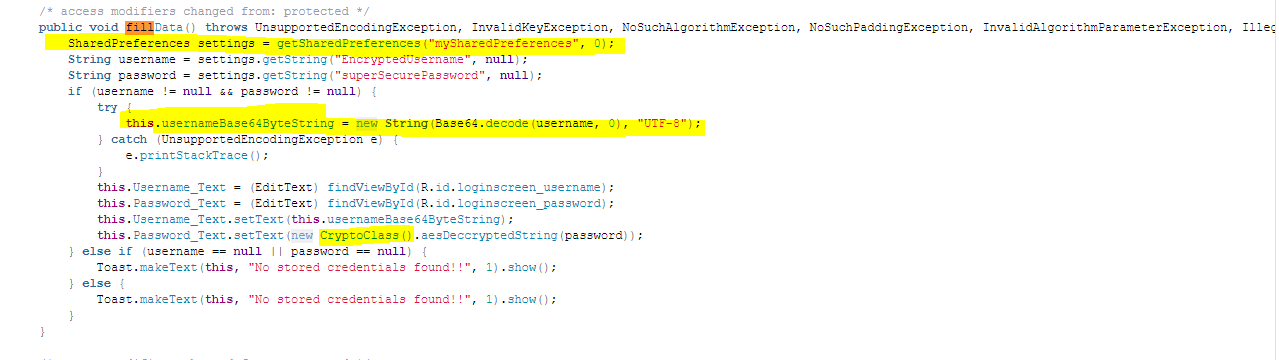
\includegraphics[scale=0.4]{./imagenes/filldata}}
    \caption{Código de DoLogin}
\end{figure}
Encontramos el método \textit{fillData()}. Este método llama a un archivo \textit{mySharedPreferences} (OWASP M2) que podíamos encontrar utilizando la herramienta de Android Debug Bridge (ADB). Por otro lado, podemos desencriptar la string \textit{SuperSecurePassword}, porque si nos vamos a la clase de \textit{CryptoClass}, encontramos que está hardcodeada la clave de encriptado. 
\begin{figure}[H]
    \centering
    \fbox{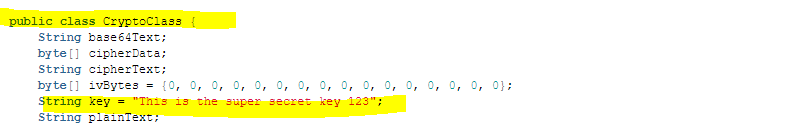
\includegraphics[scale=0.5]{./imagenes/cryptoclass}}
    \caption{Código de CryptoClass}
\end{figure}

\subsubsection{Comunicaciones}
Podemos identificar las conexiones que realizará la aplicación en este paso. Revisaremos las clases que usen \textbf{postData}
\begin{figure}[H]
    \centering
    \fbox{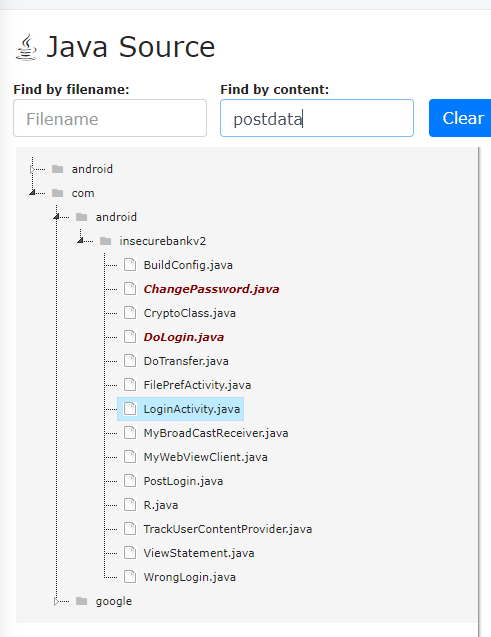
\includegraphics[scale=0.4]{./imagenes/postdata}}
    \caption{Búsqueda de posts}
\end{figure}
Podemos observar que en ámbos casos se usa un protocolo HTTP, no seguro (OWASP M3):
\begin{figure}[H]
    \centering
    \fbox{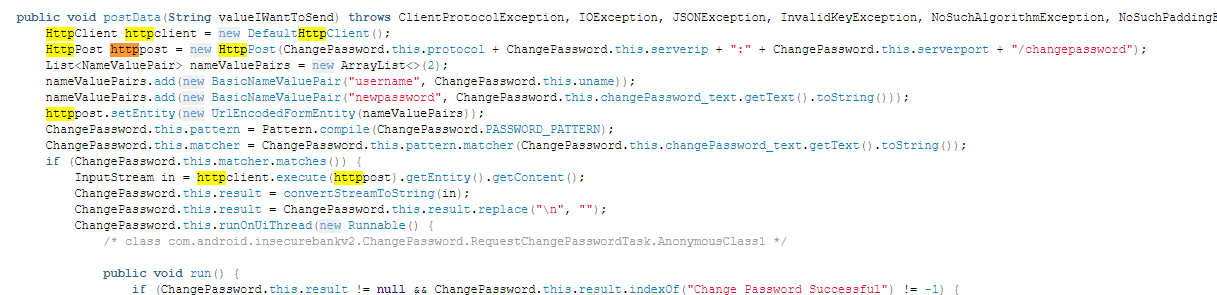
\includegraphics[scale=0.4]{./imagenes/http_changepassword}}
    \caption{Código de ChangePassword}
\end{figure}
\begin{figure}[H]
    \centering
    \fbox{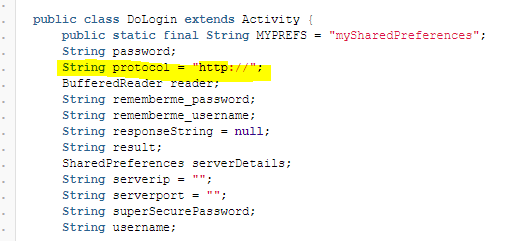
\includegraphics[scale=0.6]{./imagenes/http_dologin}}
    \caption{Código de DoLogin}
\end{figure}

Esto también ocurre en la clase \textbf{DoTransfer}, que utiliza un HttpPost con protocolo HTTP.
\begin{figure}[H]
    \centering
    \fbox{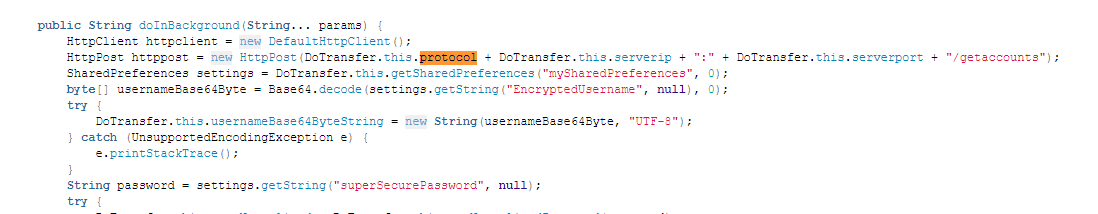
\includegraphics[scale=0.45]{./imagenes/http_dotransfer}}
    \caption{Código de DoTransfer}
\end{figure}
\subection{Análisis dinámico}
Si arrancamos la aplicación 
\begin{figure}[H]
    \centering
    \fbox{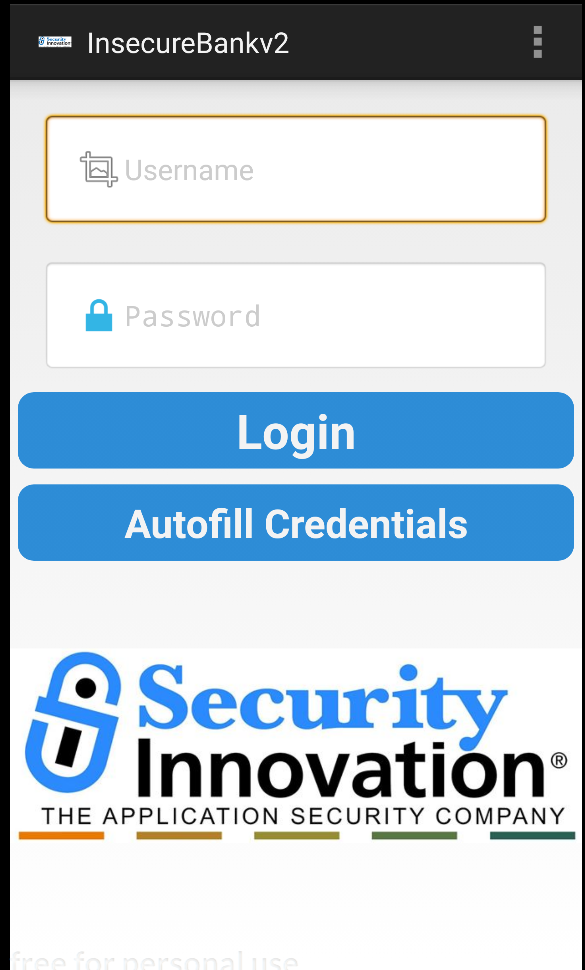
\includegraphics[scale=0.35]{./imagenes/insecurebank_1}}
    \caption{Inicio de InsecureBank}
\end{figure}
y la configuramos para que apunte al servidor donde hemos levantado el backend de python (para más información revisar la documentación de InsecureBankv2)
\begin{figure}[H]
    \centering
    \fbox{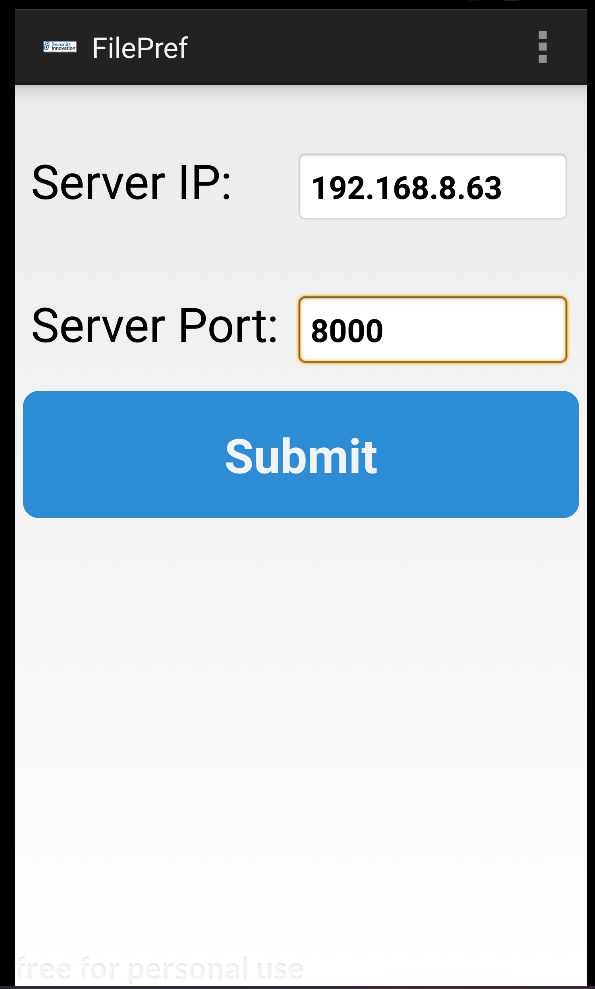
\includegraphics[scale=0.35]{./imagenes/insecurebank_2}}
    \caption{Configuración de InsecureBank}
\end{figure}
Podremos analizar las comunicaciones con wireshark. En esta caso interceptamos una petición de login con el usuario \textit{user}  y contraseña por  \textit{passwd}
\begin{figure}[H]
    \centering
    \fbox{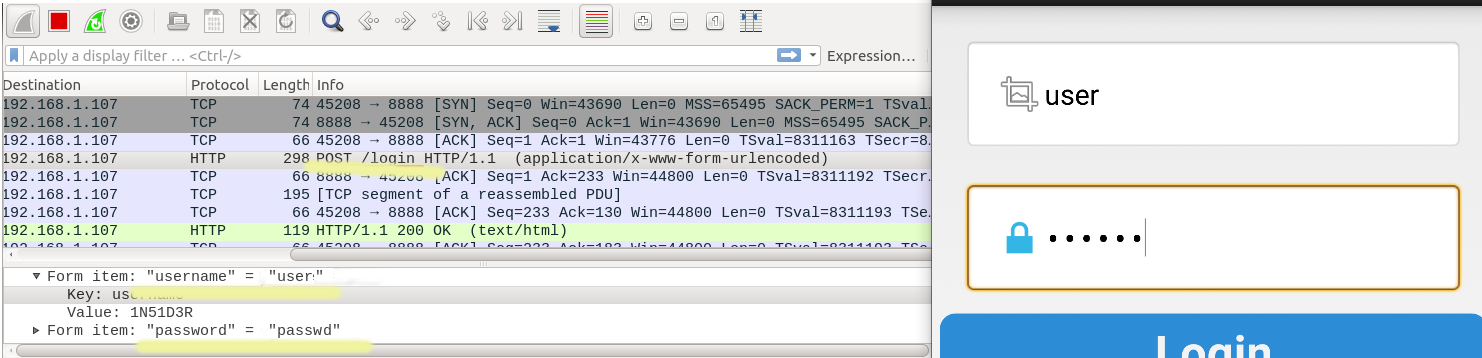
\includegraphics[scale=0.4]{./imagenes/analisisdinamico_2}}
    \caption{Configuración de InsecureBank}
\end{figure}
y podemos ver que no está cifrado, al enviarse por protocolo HTTP (OWASP M4)

\newpage
% ------------------------------------------------- % 
% -              Análisis de instagram            - %
% ------------------------------------------------- % 
\section{Análisis de Instragram}
Descargamos la apk oficial de Google de esta conocida red social. 
En primer lugar, hacemos el análisis con VirusTotal.
\begin{figure}[H]
    \centering
    \fbox{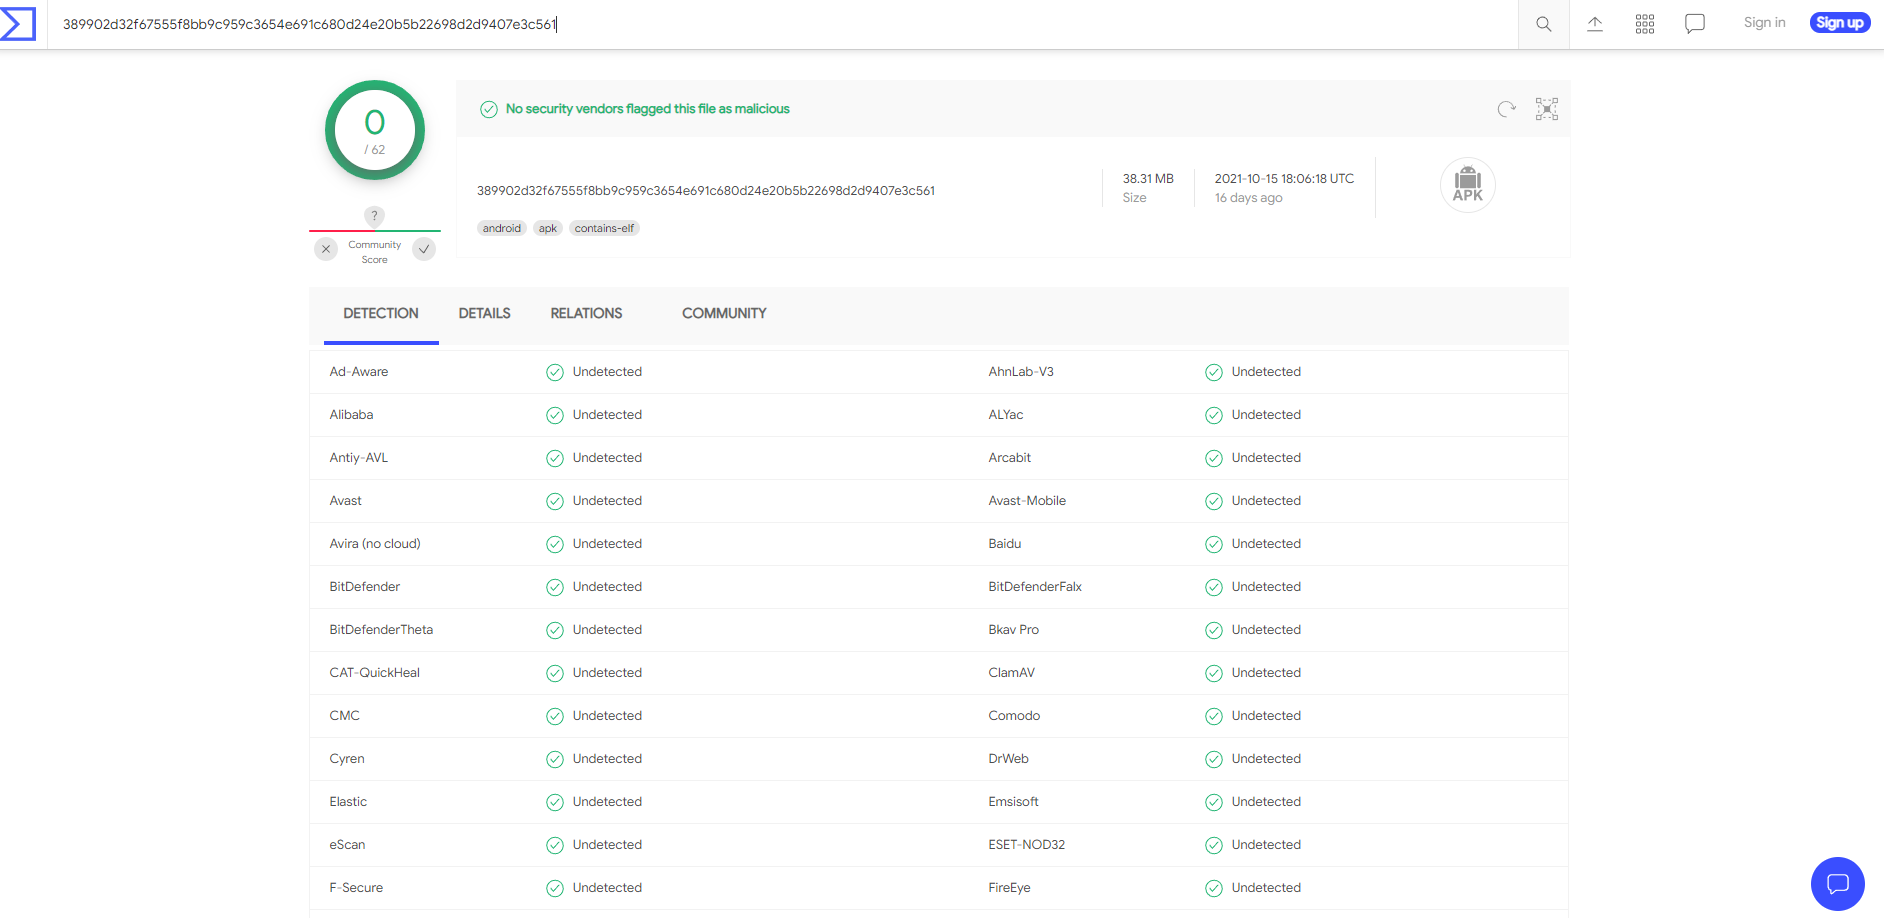
\includegraphics[scale=0.30]{./imagenes/virustotal_instagram}}
    \caption{Análisis VirusTotal}
\end{figure}

% ------------------------------------------------- % 
\subsection{Análisis estático}
\subsubsection{Permisos}
Revisemos en primer lugar el AndroidManifest.xml en búsqueda de permisos \textit{sospechosos}. 
\begin{figure}[H]
    \centering
    \fbox{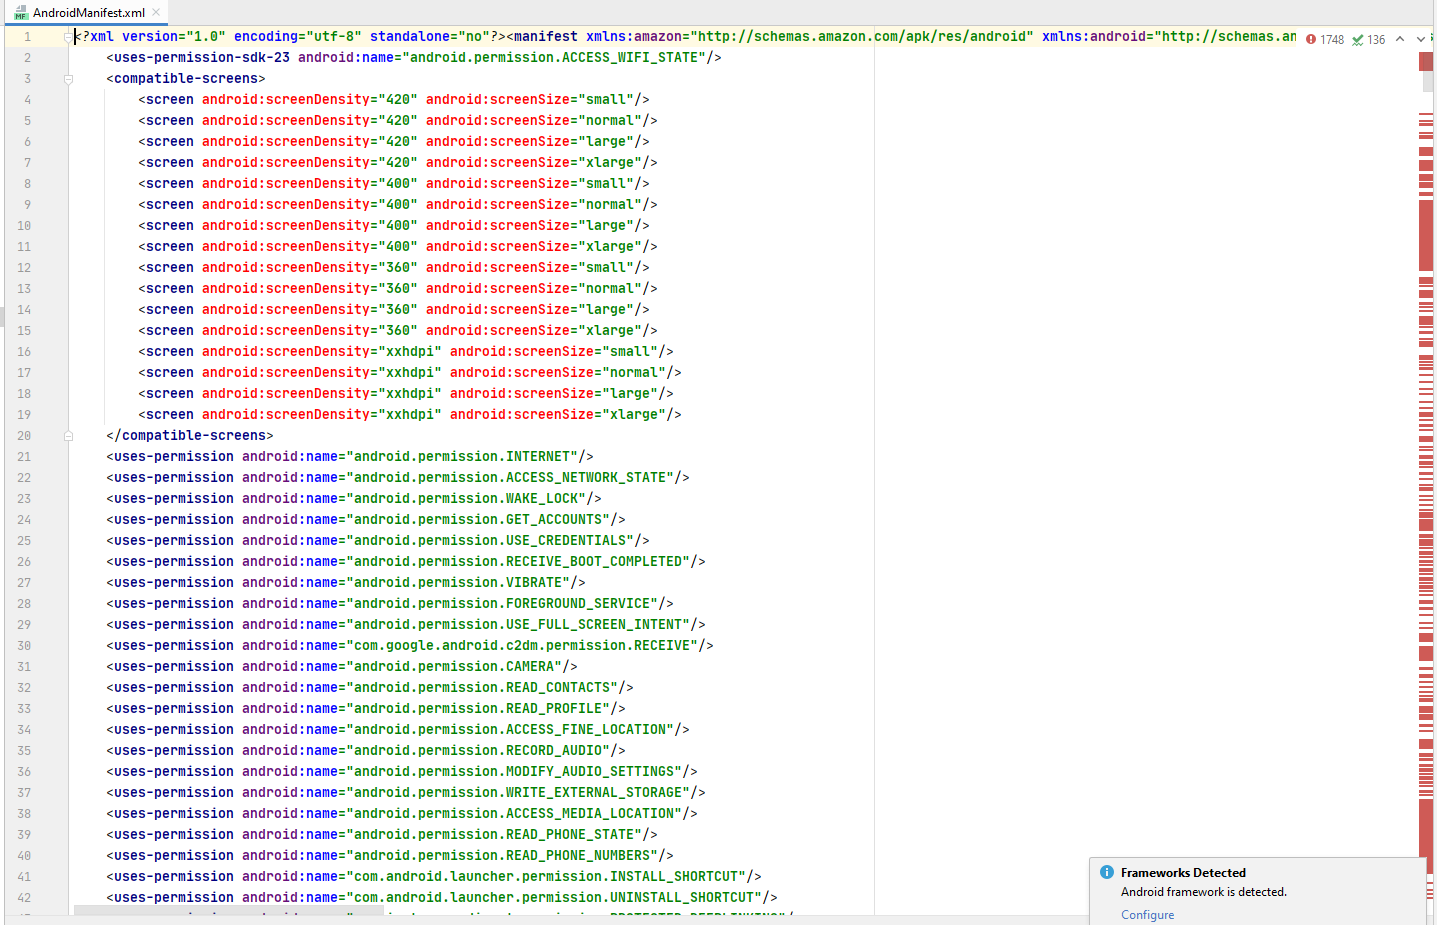
\includegraphics[scale=0.35]{./imagenes/androidmanifest_instagram}}
    \caption{AndroidManifest de Instagram}
\end{figure}
En este caso, analizaremos la aplicación utilizando AndroidStudio, tras crear los binarios con apktool, básicamente porque MobSF, por algún motivo, no es capaz de procesarla.

\begin{itemize}
    \item \textbf{WRITE\_EXTERNAL\_STORAGE}:Escrirtura en almacenamiento externo. Otras apps pueden beneficiarse de esto, sobreescribiendo o leyendo datos.
    \item \textbf{ACCESS\_MEDIA\_LOCATION}: Permie acceder a la localización de archivos multimedia. 
    \item \textbf{GET\_ACCOUNTS}: Permite a la aplicación obtener las cuentas conocidas almacenadas en el teléfono, como por ejemplo cuentas creadas por otras aplicaciones, es decir, podría obtener nuestros usuarios de otras aplocaciones.
    \item \textbf{READ\_CONTACTS}: Podrá leer los contactos almacenados en el teléfono, llamadas, correos enviados.... Esto permitiría que pueda recabar los datos del usuario y robarlos.
\end{itemize}
\subsubsection{Actividades}
No se observan actividades peligrosas.
\begin{itemize}
    \item com.instagram.mainactivity.LauncherActivity. Esta actividad está exportada, haciendo que se pueda usar por otras aplicaciones.
\end{itemize}
\subsubsection{Receivers}
No se observan \textit{recibidores} peligrosos.
\subsubsection{ContentProvider}
No se observan ContentProviders peligrosas.
\subsubsection{Almacenamiento de credenciales}
Las credenciales se almacenan de forma segura, si revisamos el \textbf{LoginActivity}, podremos ver que Instagram funciona a través de un servidor externo de Python, al cual manda los datos de forma cifrada:
\begin{figure}[H]
    \centering
    \fbox{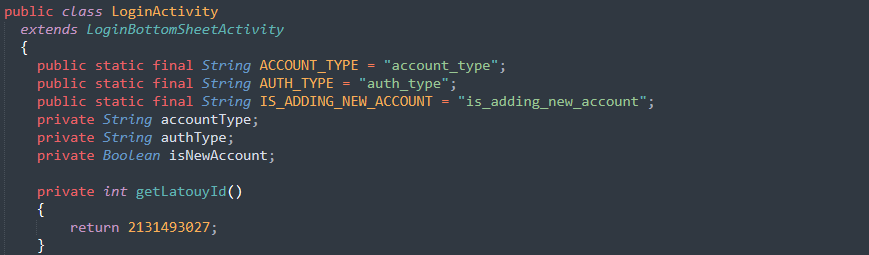
\includegraphics[scale=0.4]{./imagenes/login_coidgo_instagram}}
    \caption{Código de Login de instagram.}
\end{figure}
\subsubsection{Comunicaciones}
Todas las comunicaciones son de la forma HTTPS.
\begin{figure}[H]
    \centering
    \fbox{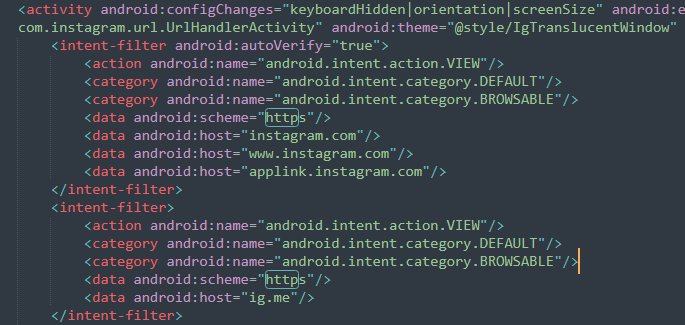
\includegraphics[scale=0.4]{./imagenes/comunicacion_https_instagram}}
    \caption{Comunicación https de Instagram.}
\end{figure}
% ------------------------------------------------- % 
\subsection{Análisis dinámico}
No se observan comportamientos anómalos en el análisis dinámico. Los datos no pueden ser interceptados con WireShark ni Burp. He probado a subir imágenes, pero Genymotion cierra la aplicación automáticamente. 

\newpage
% ------------------------------------------------- % 
% -          Análisis de MyFitnessPal             - %
% ------------------------------------------------- % 
\section{Análisis de MyFitnessPal}
En este punto, usaremos el la aplicación \textit{creackeada} descargada de un repositorio no oficial. Además, compararemos con su versión oficial. Esta aplicación sirve para contar calorías, y ver los planes nutricionales.
\subsection{Análisis estático}
En primer lugar, se observa que la versión oficial tiene un tamaño de 24MB frente a los 70MB de la versión \textit{creackeada}.
Veamos el análisis con VirusTotal de la aplicación \textit{creackeada}.
\begin{figure}[H]
    \centering
    \fbox{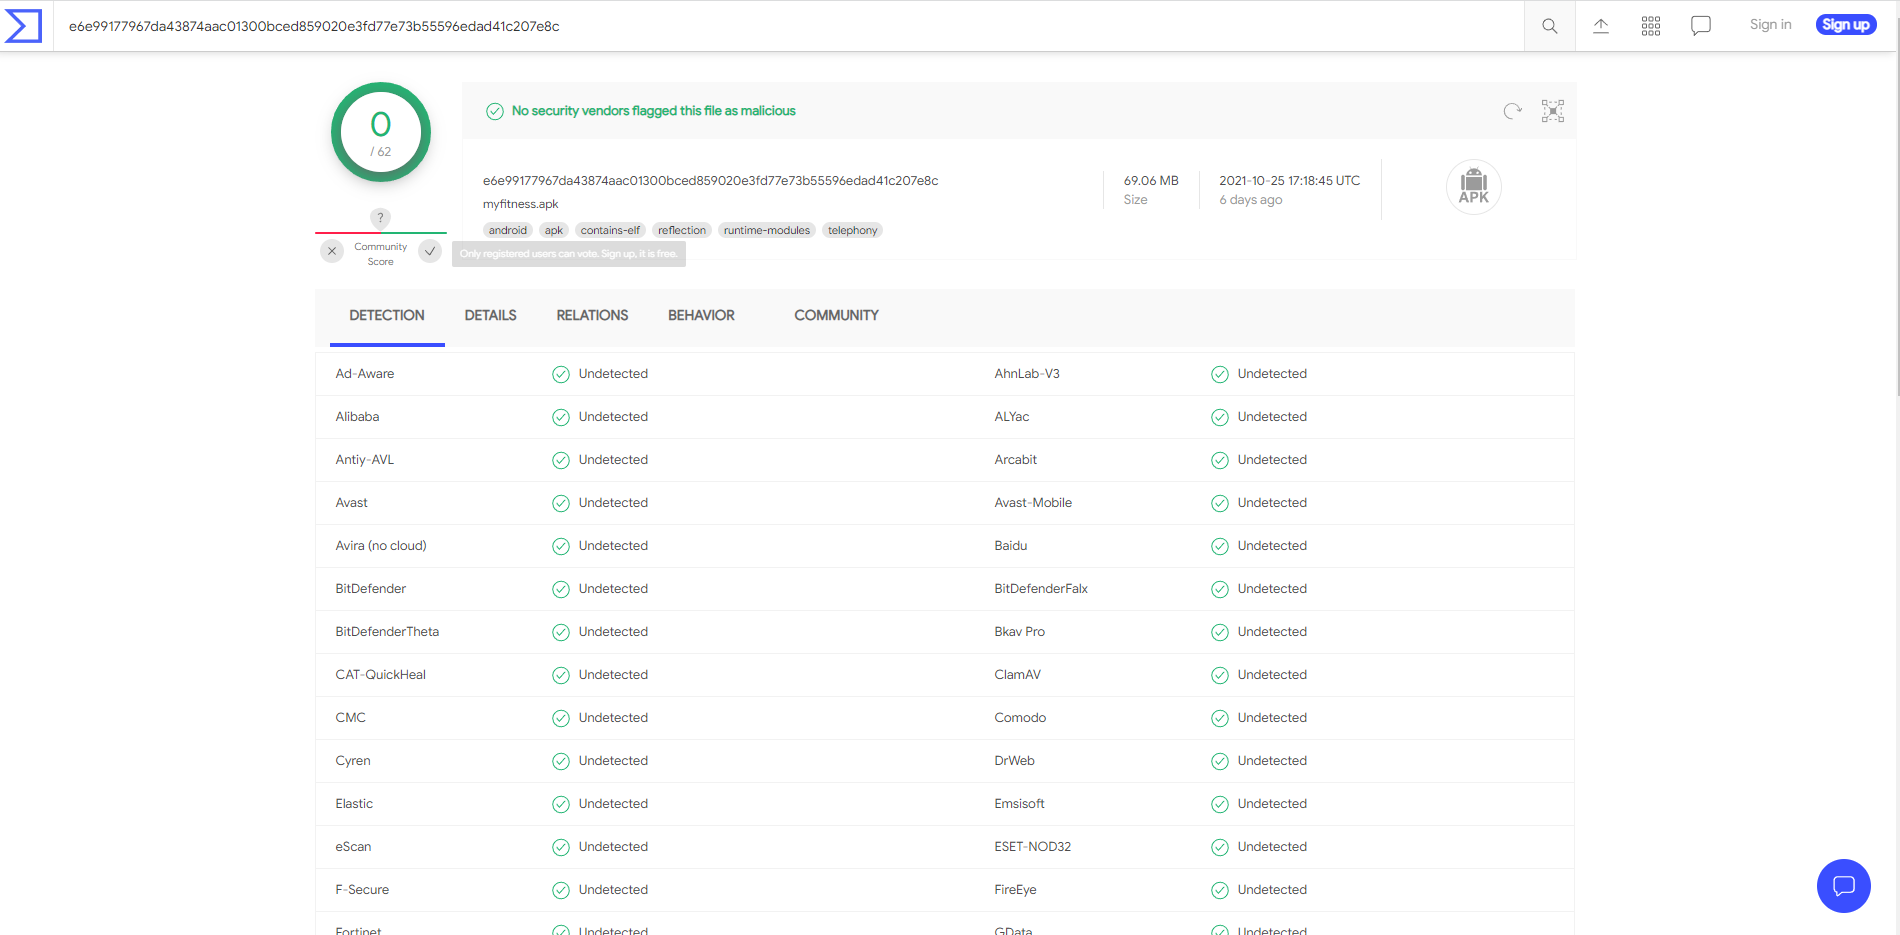
\includegraphics[scale=0.35]{./imagenes/virustotal_myfitnesspal}}
    \caption{Comunicación https de Instagram.}
\end{figure}
\subsubsection{Permisos}
Ambas aplicaciones utilizan prácticamente los mismos permisos, sin embargo, la aplicación crackeada utiliza
\begin{itemize}
    \item \textbf{android.permission.READ\_PHONE\_STATE}: Permite a la aplicación acceder al número de teléfono, número de serie, llamadas activas... Un permiso que no debería necesitar una aplicación de deporte.
\end{itemize}
\subsubsection{Actividades}
La aplicación  original tiene una actividad que conecta con \textit{Amazon Mobile Ads}, que no encontramos en la versión creackeada.
\begin{figure}[H]
    \centering
    \fbox{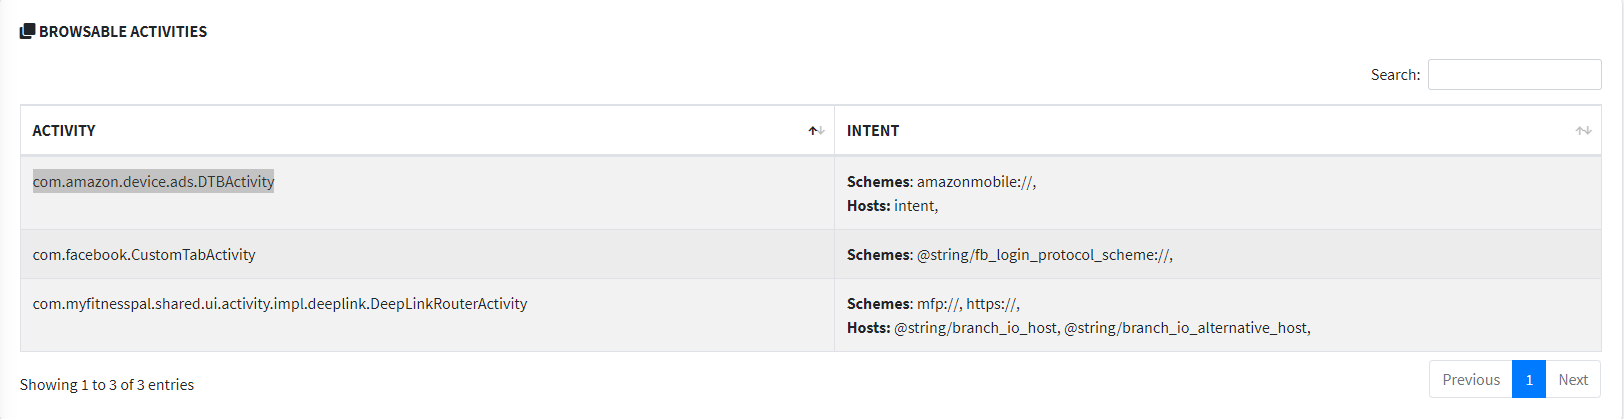
\includegraphics[scale=0.35]{./imagenes/actividades_mfp}}
    \caption{Actividades de MyFitnessPal.}
\end{figure}
\begin{figure}[H]
    \centering
    \fbox{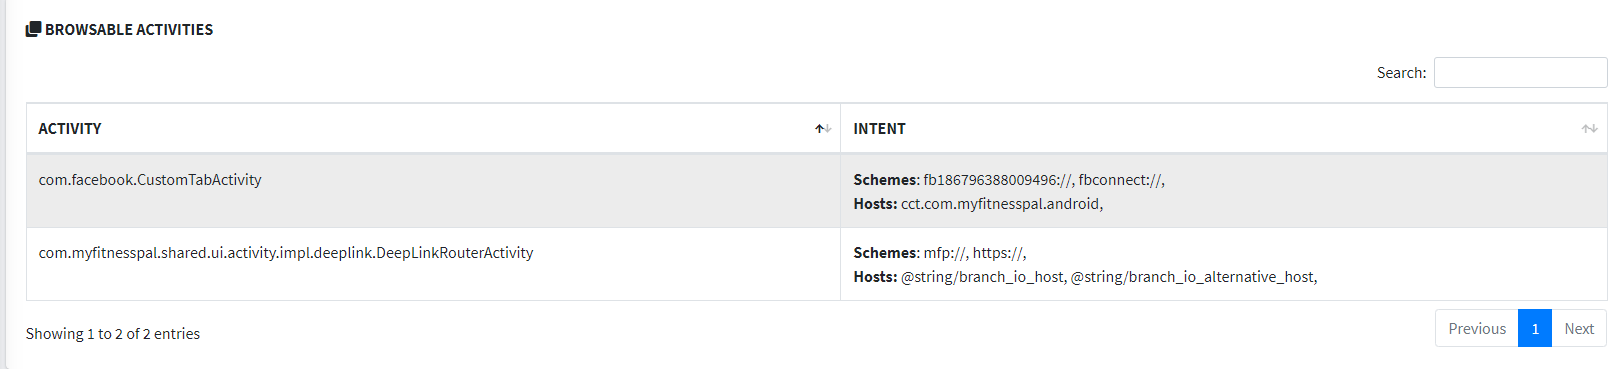
\includegraphics[scale=0.35]{./imagenes/actividades_mfp_crack}}
    \caption{Actividades de MyFitnessPal crack.}
\end{figure}
\subsubsection{Receivers}
No se encuentran Receivers peligrosos, pero sí diferentes: la versión crackeada utiliza en Adsbynimbus, pero no hay anuncios mostrados por pantalla al utilizarla. Aunque ambas tienen distintos Receivers sin protección de permisos.
\begin{figure}[H]
    \centering
    \fbox{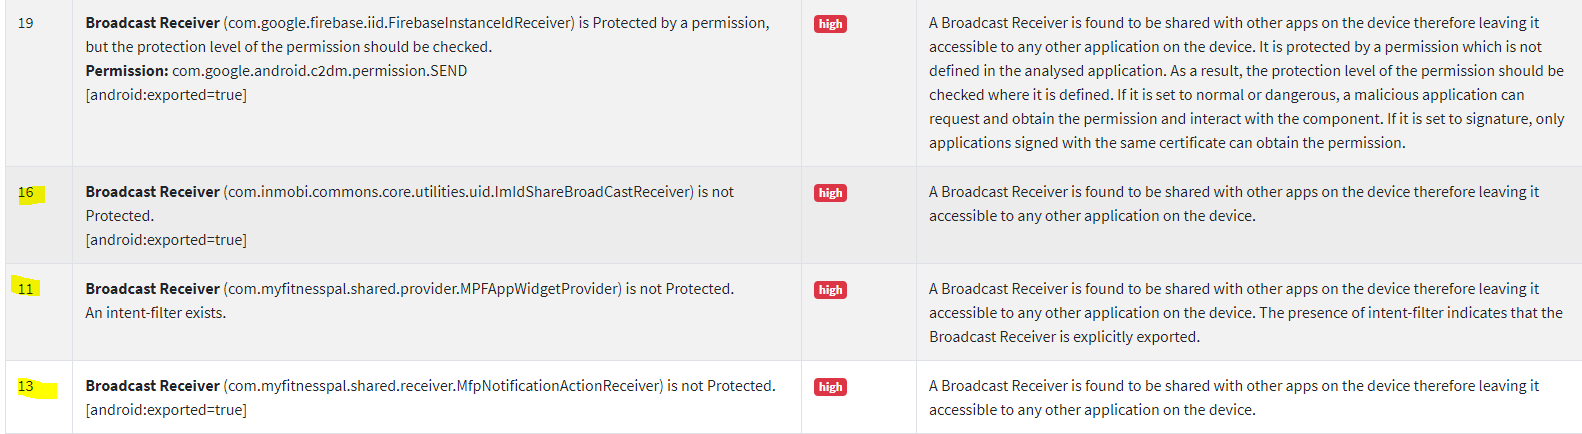
\includegraphics[scale=0.38]{./imagenes/receiver_sin_proteccion}}
    \caption{Receiver de MyFitnessPal}
\end{figure}
Pero no hay nada interesante si revisamos el código, solo notificaciones.
\begin{figure}[H]
    \centering
    \fbox{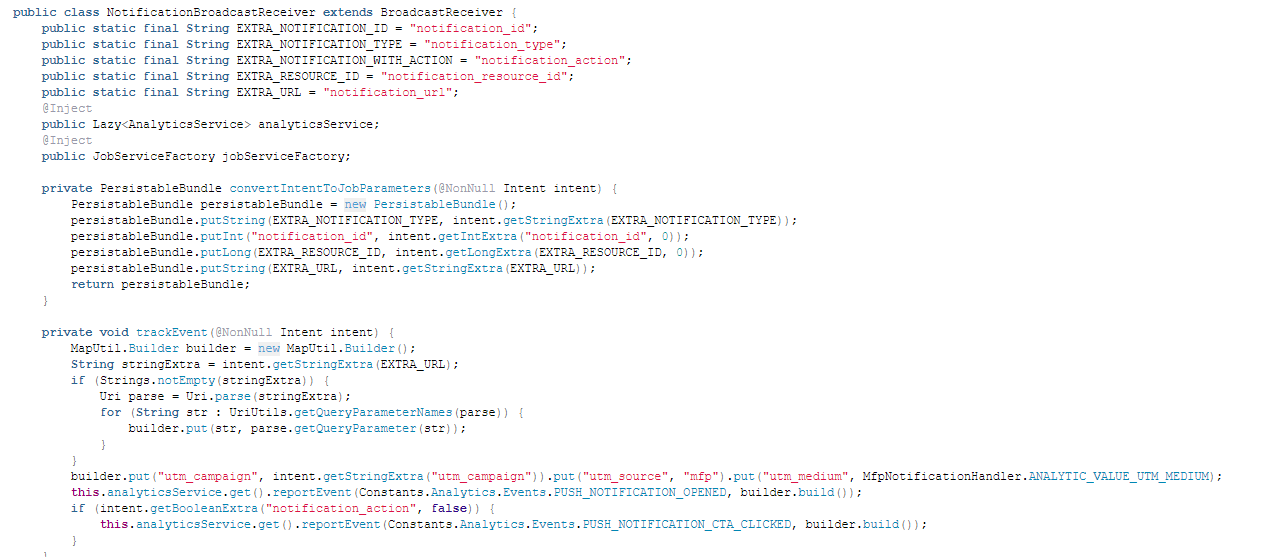
\includegraphics[scale=0.4]{./imagenes/notification}}
    \caption{Código del Receiver}
\end{figure}
\subsubsection{ContentProvider}
Podemos observar que la aplicación crackeada, contiene un ContentProvider, \textbf{com.myfitnesspal.shared.api.auth.IdentityContentProvider}, que no está protegido y que tampoco aparece en la aplicación original. Pero revisando los códigos, vemos que simplemente es un ContentProvider con otro nombre, aunque con una dependencia menos. 
\begin{figure}[H]
    \centering
    \fbox{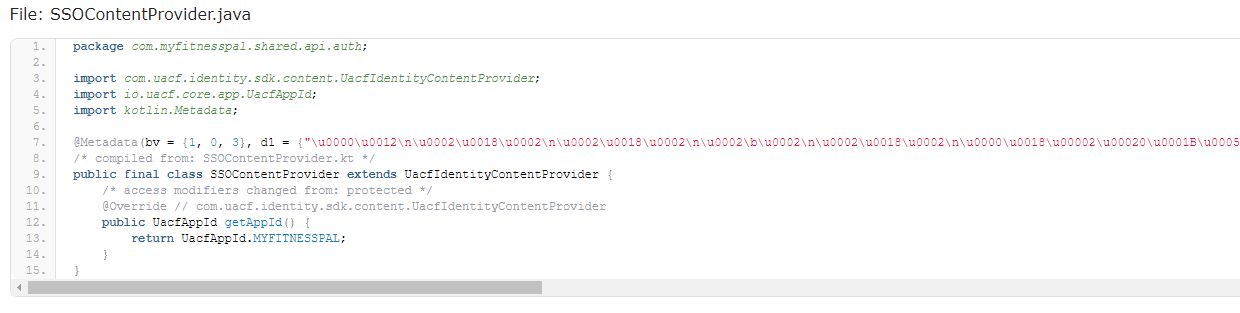
\includegraphics[scale=0.4]{./imagenes/ssocontent}}
    \caption{SSOContentProvider}
\end{figure}
\begin{figure}[H]
    \centering
    \fbox{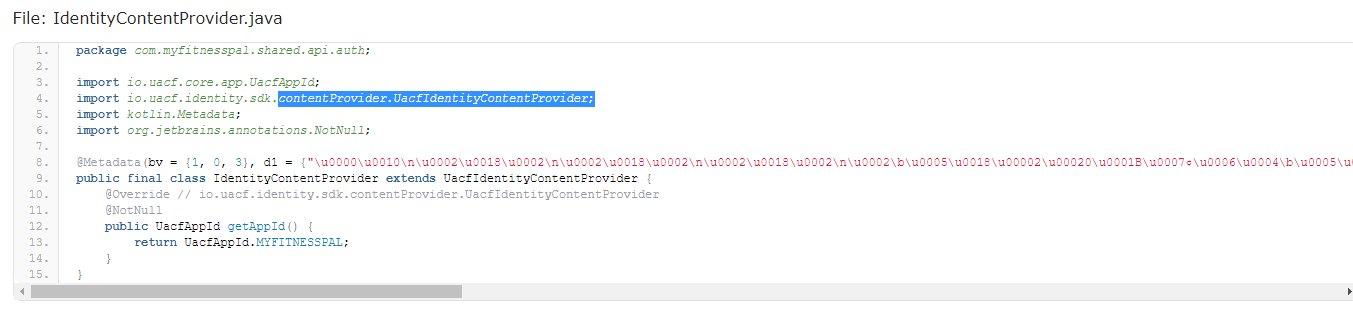
\includegraphics[scale=0.4]{./imagenes/identity}}
    \caption{IdenttyContentProvider, creackeado.}
\end{figure}

\subsubsection{Almacenamiento de credenciales}
No he conseguido encontrar los archivos de almacenamiento de credenciales. Sin embargo, ambas aplicaciones utilizan SQLite y ejecuta SQL sin sanitizar. 
Sí que podemos ver que los parámetros como la contraseña son privados.
% ------------------------------------------------- % 
\subsection{Análisis dinámico}
Al utilizar las aplicaciones en Genymotion y Santoku, se cerraban automáticamente. Quizá por ser versiones antiguas o por RAM, así que decidí probar ambas versiones en un Samsung Galaxy A5 que tengo para emergencias. A primera vista las aplicaciones son iguales, con la diferencia de que la apliacción crackeada, al instalarse, instala también la aplicación \textbf{Aptoide}, la cual al desinstalarse, provoca que la aplicacón crackeada no funcione más.\\
Si accedemos a ella, veremos que a diferencia de la original, tendremos disponibles todas las herramientas premium y no habrá anuncios. \\
De todas formas, no es recomendable el uso de este tipo de aplicaciones, ya que  nada es gratis, y probablemente esté leyendo y utilizando nuestros datos (mejor dicho, comerciando) con terceros. 

\newpage
% ------------------------------------------------- % 
% -                     Anexos                    - %
% ------------------------------------------------- % 
\section{Anexos}
\subsection{Problemas de versionado}
En caso de querer replicar el estudio aquí hecho, hay que tener cuidado. Muchas de las herramientas utilizadas usan \textit{python}, además, el backend de InsecureBankV2 es un archivo python también. El problema es el siguiente: las herramientas necesitan que se use de python3 en adelante y el backend de InsecureBankv2 requiere de python2, o no se ejecutará correctamente.\\
También da problemas similares \textit{Androl4b} y \textit{Genyotion}. Recomiendo encarecidamente hacer estos tests sobre una máquina Linux montada en una máquina virtual, ya que nos dará (como norma general) mayor facilidad de uso que montar nuestor lab en Windows, al menos desde mi experiencia. 
\subsection{Lista de OWASP TOP 10 MOBILES RISKS}
\begin{itemize}
    \item M1 - Improper Platform Usage
    \item M2 - Insecure Data Storage
    \item M3 - Insecure Communication
    \item M4 - Insecure Authentication
    \item M5 - Insufficient Cryptography
    \item M6 - Insecure Authorization
    \item M7 - Client Code Quality
    \item M8 - Code Tampering
    \item M9 - Reverse Engineering
    \item M10 - Extraneous Functionality
\end{itemize}

\subsection{Análisis de riesgos OWASP con Quixxi}
Añado los resultados de los tests que ejecuta Quixxi para determinar las vulnerabilidades. En principio esto iba a ser una subsección de cada una de las aplicacicones, pero al ver que la aplicación de Instagram, que en un principio es segura y conocida pasaba menos test que la aplicación InsecureBank, preparada para ser insegura, he pensado que quizá no son tests demasiado fiables.\\
Adjunto tablas:
\begin{figure}[H]
    \centering
    \fbox{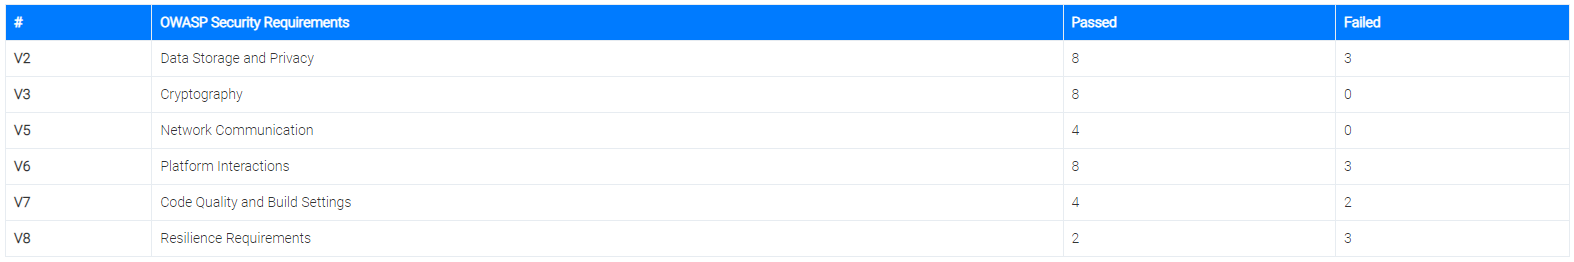
\includegraphics[scale=0.38]{./imagenes/owasp_insecurebank_1}}
    \caption{Tabla resumen InsecureBank}
\end{figure}

\begin{figure}[H]
    \centering
    \fbox{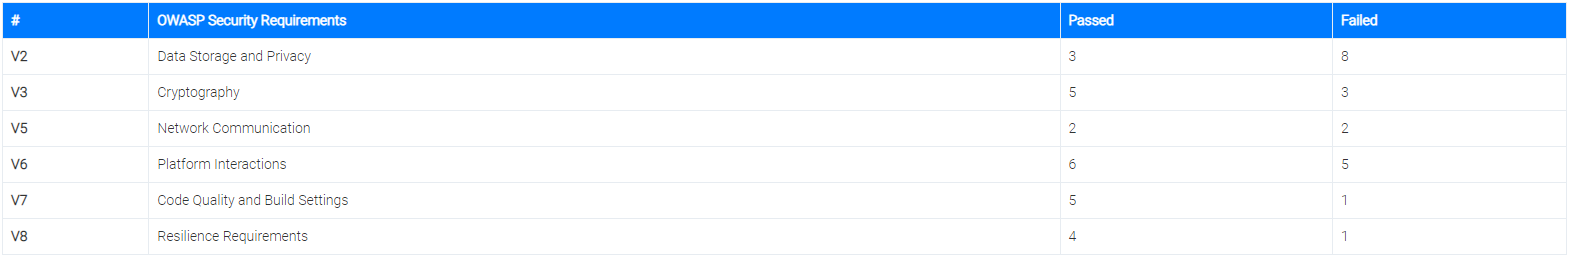
\includegraphics[scale=0.38]{./imagenes/owasp_myfitnesspal_1}}
    \caption{Tabla resumen MyFitnessPal}
\end{figure}

\begin{figure}[H]
    \centering
    \fbox{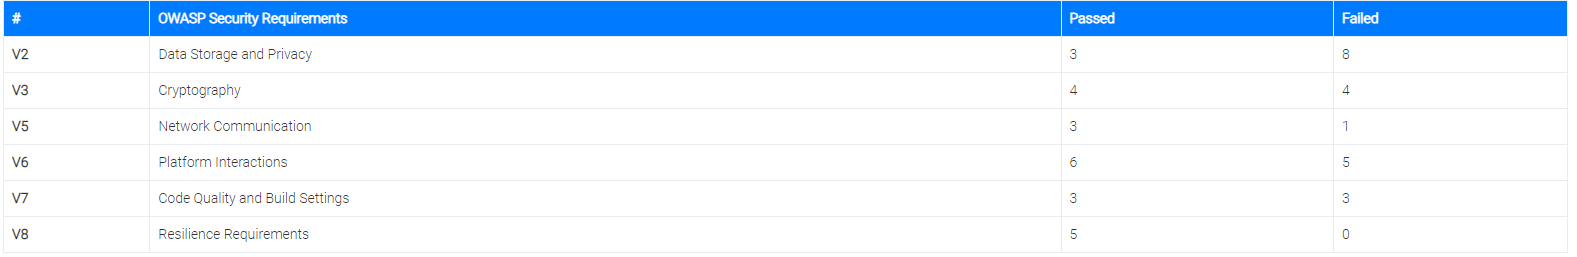
\includegraphics[scale=0.38]{./imagenes/owasp_instagram_1}}
    \caption{Tabla resumen Instagram}
\end{figure}
\end{document} 
